\documentclass{standalone}

\usepackage{tikz,tikz-3dplot, tkz-euclide}
\usetikzlibrary{arrows.meta}
\tikzset{>={Latex[round]}}
\usepackage{pgfplots}
\pgfplotsset{compat=1.12}
\usepgfplotslibrary{fillbetween}

\begin{document}

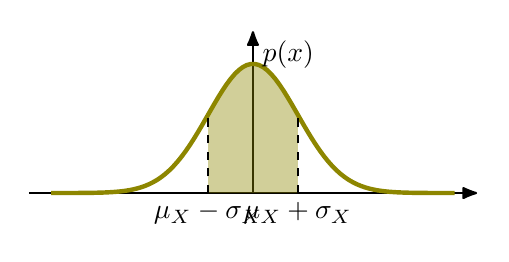
\begin{tikzpicture}
    \begin{axis}[
                    ymax=0.5,
                    axis lines=middle,
                    axis line style={thick, ->},
                    width=.6\textwidth,
                    height=.3\textwidth,
                    ytick=\empty,
                    xtick=\empty,
                    xmin=-5,
                    xmax=5,
                    ylabel=$p(x)$, 
                    clip=false]
        \addplot[name path=gaussian, olive, ultra thick, samples=100, domain=-4.5:4.5] {1/((2*pi)^(1/2))*e^(-x^2 / 2)};
        \path[name path=axis] (-5,0) -- (5,0);
        \addplot[olive, fill opacity=0.4] fill between[of=gaussian and axis, soft clip={domain=-1:1}];
        \addplot[thick, dashed] coordinates {(1,0) (1, 0.241970725)};
        \addplot[thick, dashed] coordinates {(-1,0) (-1, 0.241970725)};
        \node at (-1, 0.0) [below] {$\mu_X - \sigma_X$};
        \node at (1, 0.0) [below] {$\mu_X + \sigma_X$};
    \end{axis}
    \end{tikzpicture}

\end{document}